\section{Research Gap}
\label{sec:researchgap}



%In der Multi-Lane-Version des Nagel-Schreckenberg-Modells (siehe \cite{multi-lane}) geben die Regeln einen Zwang zum Einleiten des Überholvorganges, wenn sich die Möglichkeit dazu ergibt, vor. Ebenso wurde für den Rückwechsel auf die Normalspur eine Wahrscheinlichkeit festgelegt.
%
%Das Verhalten des Entscheiders Mensch, was auch im Straßenverkehr eine große Rolle spielt, wurde bisher eher als eine Art \enquote{Black Box} betrachtet. 
%Jeder Fahrzeugführer trifft zu jedem Zeitpunkt unter gleichen Voraussetzungen die gleiche Entscheidung. 
%Dies ist aber in der Realität nicht so. 
%Ein Fahrer kann z. B. vorsichtiger sein als ein anderer und, trotz des gleichen Abstands und der gleichen Geschwindigkeiten, auf ein Überholmanöver verzichten, weil er seine Umwelt anders einschätzt.
%
%In \cite{dat-ba} wird der Hang zum Wechsel oder zur Beibehaltung der Spur nicht nur durch fest vorgegebene Wahrscheinlichkeiten simuliert, sondern durch individuell für jedes Fahrzeug zu jedem Zeitschritt berechnete \enquote{Kräfte}, deren \enquote*{Entscheidung}, durch entsprechende berechnete Wahrscheinlichkeiten getragen, mehr oder weniger häufig zur Ausführung kommen. 
%Durch die gezielte Beachtung des umgebenden Verkehrs und das Bewerten der zur Wahl stehenden Alternativen soll es nun möglich sein, das menschliche Verhalten besser als bisher abzubilden.
%
%Das Hauptaugenmerk von \cite{dat-ba} lag auf der theoretischen Modellentwicklung/""Modellierung. 
%Eine praktische Umsetzung und somit die Kontrolle des Erdachten und natürlich die Möglichkeit eines Vergleichs zwischen dem neuen Ansatz und bereits existierenden Modellierungen, z. B. dem Mehrspurmodell aus \cite{multi-lane}, ist bisher nicht durchgeführt worden. 
%Dies ist Ziel dieser Arbeit.
%
%\subsection*{Mögliches Problem}
%\addcontentsline{toc}{subsection}{Mögliches Problem}
%
%Aus der Art und Weise, wie der Ansatz in das ursprüngliche Modell nach \cite{na-sch} (und nicht in die Mehrspurvariante nach \cite{multi-lane}) integriert wurde, könnte ein Problem entstehen.
%Eine der drei Regeln, die die Kollisionsfreiheit sichern sollen - das Abbremsen - wurde entfernt und durch das \enquote{Social-Force-Modell} ersetzt (siehe \cite{dat-ba}, S. 21 \& Abb. 16, bzw. Vortragsfolien S. 7).
%Dies kann dazu führen, dass in der Simulation ein Auffahrunfall unausweichlich ist.
%Auch wenn Verkehrsunfälle in der realen Welt durchaus vorkommen, sollte man sie in dieser Simulation nicht provozieren. Zudem ist die Unfallhäufigkeit so gering, dass sie bei betrachteter Zeitspanne und Streckenlänge unbedeutend ist.
%
%\begin{figure}[hptb]
% \centering
% 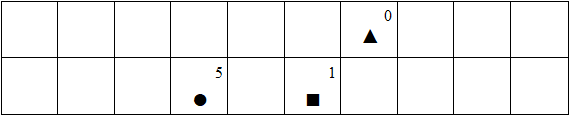
\includegraphics[width=0.6\textwidth]{problem-beispiel}
% \caption[Problem-Beispiel]{Beispiel für ein Problem-Szenario, drei Fahrzeuge und deren Geschwindigkeiten}
% \label{figure:problem-beispiel}
%\end{figure}
%
%\noindent
%In \cref{figure:problem-beispiel} würde dem Fahrzeug $\bullet$ nach dem Multi-Lane-Modell aus \cite{multi-lane} das Ausscheren vorgegeben, denn die linke Spur bietet mehr Platz als die rechte und es gibt keinen nachfolgenden Verkehr auf der anderen Spur. 
%Fahrzeug $\blacktriangle$ ist $j=3$ Felder vor $\bullet$.
%Ein Abbremsen von $\bullet$ auf $v_{\bullet}=j-1=2$ würde veranlasst.
%Dass $\blacktriangle$ gleichzeitig um $1$ beschleunigen könnte, spielt keine Rolle. \\
%Nach dem \enquote{Social-Force-Modell} würde für das Fahrzeug $\bullet$ wahrscheinlich eine höhere Kraft der entsprechenden Zelle und somit Wahrscheinlichkeit für das Ausscheren berechnet werden.
%Dies muss aber nicht zur Entscheidung in Richtung Spurwechsel führen.
%$\blacksquare$ kann im aktuellen Zeitschritt max. auf $v_{\blacksquare}=2$ beschleunigen, $\blacktriangle$ max. auf $v_{\blacktriangle}=1$.
%Da Fahrzeug $\bullet$ seine Geschwindigkeit aber nur durch die Zufallsgröße \enquote{Trödeln} um max. $1$ reduzieren könnte, würde es beim Simulationsschritt \enquote{Fahren} auf das gleiche Grid-Feld oder gar davor gesetzt werden. \\
%Da ein solches Szenario insbesondere bei Stockungen und an Stauenden auftreten dürfte, wären dort Auffahrunfälle unvermeidbar. 
%
%Das \enquote{Social-Force-Modell} wird im normalen Verkehrsfluss einen Teil der möglichen Unfallszenarien durch Ausweichen verhindern, aber bei \enquote*{Auswahl} der weniger wahrscheinlichen Alternative geradeaus zu fahren, wird sich das fehlende \enquote*{Bremsen} bemerkbar machen.
